\newpage
% neuer Layer für Geländeplan
\DeclareNewLayer[background, oddorevenpage,  width=125mm,%
height=169mm, contents={%
  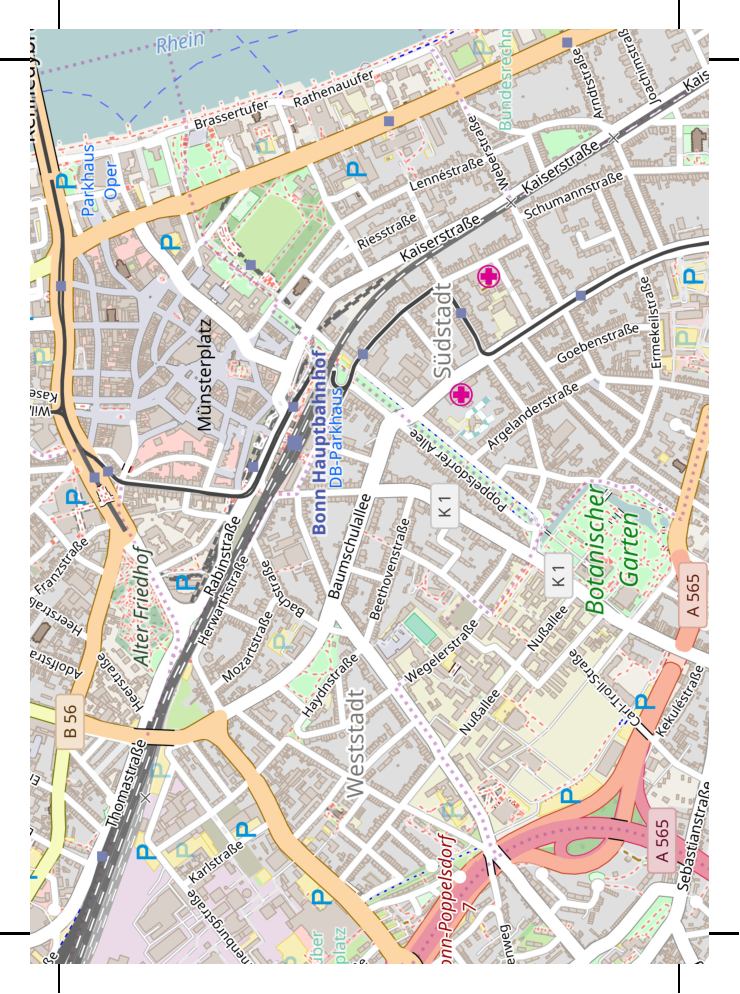
\includegraphics{wallpaper/stadtplan.pdf}%
}]{raumplana6}
\newpairofpagestyles[scrheadings]{raumplan}{}
\AddLayersAtBeginOfPageStyle{raumplan}{raumplana6}
\pagestyle{raumplan}
\null
\label{uebersichtskarte}

\newpage
\section*{Impressum}
\label{impressum}
\pagestyle{cropmarksstyle}

\RaggedRight
{\small
Die FOSSGIS 2018 wird gemeinsam vom FOSSGIS e.V. und der Universität Bonn organisiert.

\vspace{0.5em}
\newlength\logoHeight
\setlength{\logoHeight}{2.5\baselineskip}
\includegraphics[height=\logoHeight]{FOSSGIS}
\hspace{1em}
\includegraphics[height=\logoHeight]{uni-bonn-geographie.pdf}

\vspace{0.5em}
\noindent Verantwortlich für den Inhalt:\\
FOSSGIS e.V.\\
Römerweg 5\\
79199 Kirchzarten

\vspace{0.5em}
\noindent Diese Programmheft wurde unter Verwendung von \LaTeX\ und 
anderer freier Software zusammengestellt.\\
Quellcode: github.com/fossgis/booklet2018\\
\noindent Satz und Layout: Michael Reichert\\
Titelgestaltung: Christopher Lorenz, Michael Reichert\\
Geodaten: \includegraphics[height=7pt]{copyright}~Open\-Street\-Map-Mitwirkende, osm.org/copyright\\
Icons in den Tabellen: SJJB Management, CC-0\\
Lektorat:
  Astrid Emde,
  Falk Zscheile,
  Frederik Ramm,
  Katja Haferkorn,
  Niklas Alt\\

\vspace{1em}
\noindent \begin{minipage}[htbp]{0.2\textwidth}
\noindent\includegraphics[width=\linewidth]{cc-by-sa-pdf}
\end{minipage}
\hfill
\begin{minipage}[hbtp]{0.74\textwidth}\RaggedRight
  {\small
    Alle Inhalte dieses Programmhefts unterliegen, sofern nicht anders angegeben,
    der Lizenz \emph{Creative Commons Namensnennung Weitergabe unter gleichen Bedingungen 3.0}.
    Logos von Firmen und Organisationen sind hiervon ausgenommen.
  }
\end{minipage}
